\documentclass[runningheads]{llncs}

\usepackage{graphicx}
% Used for displaying a sample figure. If possible, figure files should
% be included in EPS format.

\begin{document}
%
\title{Simulation Paper}

\author{Benjamin Vandersmissen\inst{1} \and
Lars Van Roy\inst{2} \and \\
Evelien Daems\inst{3} \and
Frank Jan Fekkes\inst{4}}
%
\authorrunning{F. Author et al.}
% First names are abbreviated in the running head.
% If there are more than two authors, 'et al.' is used.
%
\institute{
\email{benjamin.vandersmissen@student.uantwerpen.be} \and
\email{lars.vanroy@student.uantwerpen.be} \and
\email{evelien.daems@student.uantwerpen.be} \and
\email{franciscus.fekkes@student.uantwerpen.be}}
%
\maketitle              % typeset the header of the contribution
%
\begin{abstract}
In this paper we will examine the Stride tool and discover its functionalities.
We will discuss some findings about the use of different parameters, populations and more.
In the end there is a briefly discussion of the performance of the program, a very important topic within computer related problems.

%\keywords{First keyword  \and Second keyword \and Another keyword.}
\end{abstract}

\section{Simulation}

\subsection{Stochastic variation}
We use the Stan (STochatsic ANalysis) controller to examine the influence of stochasticity on the results obtained from the simulation. \newline
In Figure \ref{fig1} the number of cummulatice cases per time-step is plotted. Here we can observe an exponantial grow of the number of cases througout time. This is not surprisingly because it can be deducted from common reason. If per time more people are affected, a larger contactpool is possibly infected. These people who are now new carriers of the disease will enter their personal contactpool and again more people will be reached.\\
Towards the end a flattening of the curve occurs. This can be explained because the population is obviously not infinite. At one point anyone who can be infected will effectively become a carrier of the disease. \newline
The same explanation can explain the curve in Figure \ref{fig2}. Now the cases are not the cummulative ones but the number of new cases in each time-step. A similar course of the curve can be observed.

\begin{figure}
	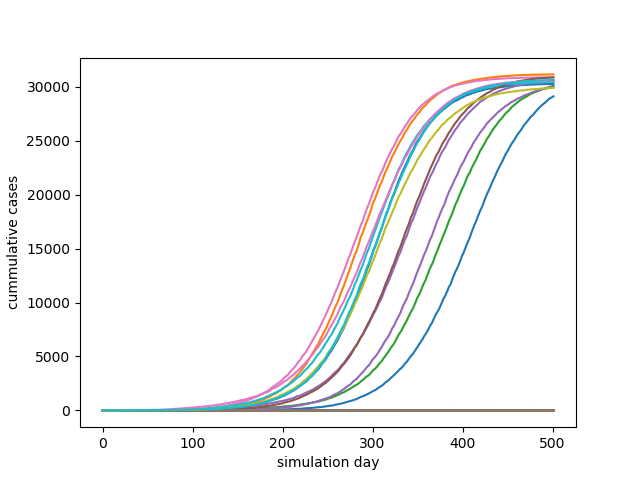
\includegraphics[width=\textwidth]{fig1.png}
	\caption{Result of a number of stochastic runs. The figure displays the distribution of the number of cummulative cases per time-step.} 	
	\label{fig1}
\end{figure}

\begin{figure}
	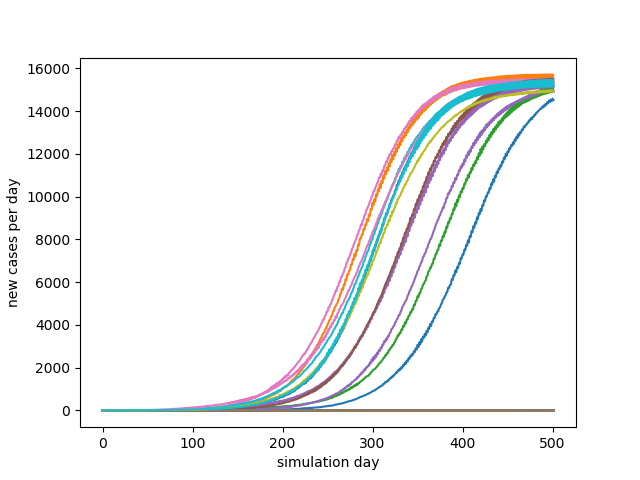
\includegraphics[width=\textwidth]{fig2.png}
	\caption{Result of a number of stochastic runs. The figure displays the distribution of the number of new cases per time-step.} 
	\label{fig2}
\end{figure}

\subsection{Determining an extinction threshold}
In the previous section 1.1 (Stochastic variation) we found that extinction will influence the outcome. It is neccessary to be able to exclusively look at outbreaks. If we can find some threshold where there is a clear difference between large outbreaks and extinctions we can seperate the two scenarios. After creating a number (50 - KAN NOG WORDEN AANGEPAST) of simulations we can plot the total number of infected cases and their occurences.  We used the file "stochastic\_analysis.xml" for the simulations. After running the simulator the outcome is plotted in the histogram "extinction\_all.jpg" where the frequency of the amount of infected cases is plotted.\\
There is a clear distinction between large outbreaks and smaller ones. The smaller ones are again plotted in the second histogram "extinction\_small.jpg". There it can be noticed that small outbreaks are really small (25 maximum). Which can be called an extinction after 500 days. The threshold can be set between than 50 and 25 000. Either of those thresholds should eliminate all extinctions in this case.\\
A very low threshold might allow some extinctions to be passed while a high threshold might eliminate an outbreak. What can be noticed is the total lack of simulations between 100 and 25000 infected cases. But there can still be exceptions in the infected cases. A threshold of 1000 would be more than adequate. It will eliminate all extinctions while keeping the outbreaks.\\
It should be noted that this threshold will change for al lot of variables. Variables like time and population will affect the threshold. A new threshold should be determined for each simulation.

\begin{figure}
	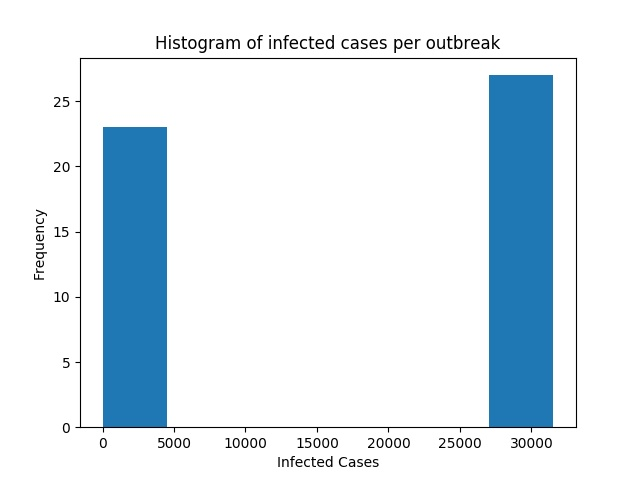
\includegraphics[width=\textwidth]{extinction_all.jpg}	
	\label{fig3}
\end{figure}

\begin{figure}
	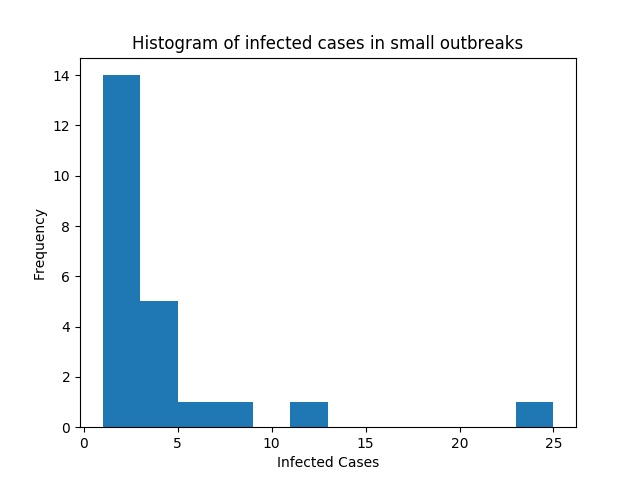
\includegraphics[width=\textwidth]{extinction_small.jpg}	
	\label{fig4}
\end{figure}


\subsection{Estimating the immunity level}
\subsection{Estimating R\textsubscript{0}}

\section{Population generation}
\subsection{Investigating the influence of demography on epidemics}
\subsection{Vaccinating on campus}
\newpage
\subsection{Is commuting to work important for disease spread?}
One could easily assume that working at a different location affects the rate at which a disease spreads, as it enhances it's reach. In a first simulation I generated simulations for 5 different commuting percentages. As you can clearly see, it does affect the rate at which the disease spreads, but it has no, or little, effect on whether the disease does or does not spread. In all cases, the entire population got the disease, be it that it took a few days longer to get to that point. Another thing we can remark is that the highest "peak" of newly diseased people is lower the lower the commuting factor gets. A possible cause of the lac of serious effect can come from the fact there are a lot of college commuters who will have the same effect as the workplace commuters. 
\begin{figure}
	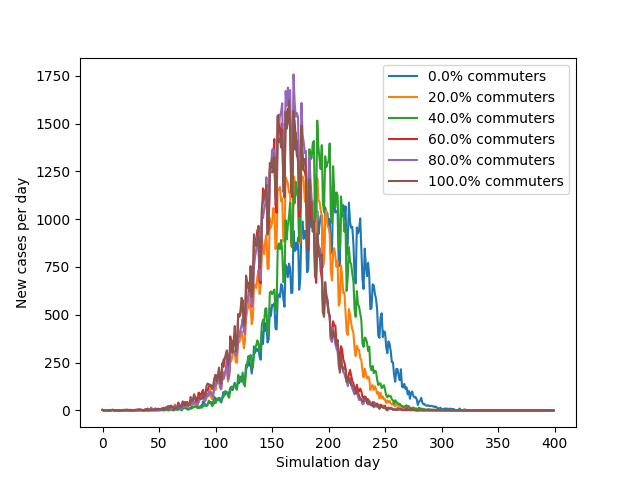
\includegraphics[width=\textwidth]{test_0-100.png}
	\caption{Results of 6 different percentages of commuters in a range from 0 to 100.}
\end{figure}
\newpage
If you watch the top of the graph, you can see that from a certain fraction and onwards, there is little to no difference in their behavior. To get a better view I graphed a closeup of percentages between 30 and 70. In the next graph you can see that the peeks are almost equally as high. You can even notice that some of the higher percentages have their peeks later then the ones with a lower percentage. 
\begin{figure}
	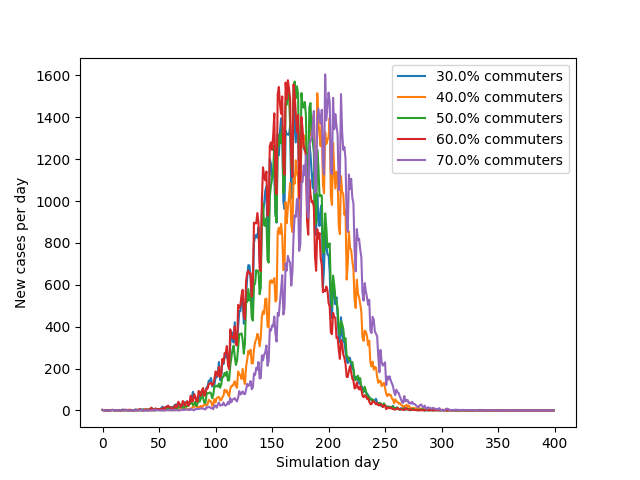
\includegraphics[width=\textwidth]{test_30-70.png}
	\caption{Results of 5 different percentages of commuters in a range from 30 to 70.}
\end{figure}
\\
Considering the recorded data we can see that solely changing the percentage of people who commute to work will not affect the spreading of disease in a significant manner. The disease will still spread all the same, but at a slower pace. 
\newpage
\section{Performance profiling of sequential code}
To study the performance of the code we will discuss a few parameters.
\\
First we will choose a random number of days to run a simulation and look at the time needed to complete the algorithm.

\begin{center}
	\begin{tabular}{ | c | c |}
	\hline
	Number of days & Time needed \\ \hline
	10 & 00:00:03:192:028 \\ \hline
	50 & 00:00:04:827:135 \\ \hline
	150 & 00:00:09:313:779 \\ \hline
	500 & 00:00:22:090:867 \\ \hline
	1000 & 00:00:39:660:327 \\
	\hline	
	\end{tabular}
\end{center}

As could be expected, there is an increase in execution time when we take a larger amount of days. But surprisingly enough is the simulation even with 1000 days rapidly. This is because after a period of time everyone will be infected and thus no further computation is necessary for the remaining amount of days. Only increasing the number of days will not make a difference in the performance of the simulation.

IMMUNITY\\
(days = 50)
\begin{center}
	\begin{tabular}{ | c | c |}
		\hline
		Immunity rate & Time needed \\ \hline
		0.2 & 00:00:04:869:367 \\ \hline
		0.4 & 00:00:04:873:811 \\ \hline
		0.6 & 00:00:04:966:409 \\ \hline
		0.8 & 00:00:05:035:361 \\ \hline
		0.99 & 00:00:04:921:399 \\
		\hline	
	\end{tabular}
\end{center} 

Varying the immunity rate, there is not a significant difference in runtime for different configurations.

When

\end{document}
